% !TeX spellcheck = en_US
\addscenariosection{1}{Clash Scenario}{Force of Will}{\images/berserk.png}

\begin{multicols*}{2}

\textbf{Author:} Shakajiub

\textbf{Source:} \href{https://discord.com/channels/740870068178649108/1237891632448278618}{Archon Studios Discord}

\textit{Wild Dragons are terrorizing the countryside.
Farmers are unable to grow their crops in peace, caravans are scared to move their goods.
You must strike at their core and defeat the beasts.
If by nothing else, then by sheer force of will.}

\subsection*{\MakeUppercase{Scenario Length}}
This Scenario is played over 12 Rounds.

\subsection*{\MakeUppercase{Player Setup}}
\textbf{Player Count:} 2 or 3

\textbf{Starting Resources:} 15 \svg{gold}, 2 \svg{building_materials}, 1 \svg{valuables}

\textbf{Starting Income:} 10 \svg{gold}, 2 \svg{building_materials}, 1 \svg{valuables}

\textbf{Starting Units:}
\begin{itemize}
  \item 2 × Few \svgunit{bronze} Units with the \textit{highest} Recruitment cost
\end{itemize}

\textbf{Town Buildings:} \svgunit{bronze} Dwelling

\textbf{Map Tile Pool:} Each player takes 1 random Far (II--III) Map Tile

\textbf{Additional Bonus:} None

\subsection*{\MakeUppercase{Map Setup}}
Take the following Map Tiles and arrange them as shown in the Scenario map layout:

\textbf{For a 2-player Scenario:}
\begin{itemize}
  \item 2 × Starting (I) Map Tile
  \item 2 × Near (IV--V) Map Tile
  \item 4 × Far (II--III) Map Tile
  \item 1 × Center (VI--VII) Map Tile, which must contain the Dragon Utopia Field
\end{itemize}

\textbf{For a 3-player Scenario:}
\begin{itemize}
  \item 3 × Starting (I) Map Tile
  \item 3 × Near (IV--V) Map Tile
  \item 6 × Far (II--III) Map Tile
  \item 1 × Center (VI--VII) Map Tile, which must contain the Dragon Utopia Field
\end{itemize}

\subsection*{\MakeUppercase{Victory Conditions}}
To win the Scenario, a Hero must Flag the Dragon Utopia Field.

\subsection*{\MakeUppercase{Defeat Conditions}}
At the end of the \nth{12} Round, if there is no winner, all players lose the Scenario.

\subsection*{\MakeUppercase{Timed Events}}

\textbf{\nth{4} and \nth{8} Rounds:}
\begin{itemize}
  \item Remove all Black cubes from every Water Wheel and Windmill on the map.
\end{itemize}

\textbf{\nth{5} and \nth{9} Rounds (2-player Scenario only):}
\begin{itemize}
  \item The second player gains 1 \svg{movement}.
\end{itemize}

\subsection*{\MakeUppercase{Additional Rules}}

During this Scenario:

\begin{itemize}
  \item When a player Visits an Obelisk, they roll 2 \svg{treasure} and choose one to resolve.
  \item A player may not use the Diplomacy card to skip Combat on the Dragon Utopia Field.
  \item When a Hero moves to the Dragon Utopia Field, they must fight, depending on chosen difficulty, the following number of Neutral Units:
  \begin{itemize}
    \item \textbf{Easy:} 1 × \svgunit{azure}, 2 × \svgunit{silver}, 1 × \svgunit{bronze}
    \item \textbf{Normal:} 1 × \svgunit{azure}, 1 × \svgunit{golden}, 2 × \svgunit{silver}
    \item \textbf{Hard:} 1 × \svgunit{azure}, 3 × \svgunit{golden}
    \item \textbf{Impossible:}  2 × \svgunit{azure}, 2 × \svgunit{golden}
  \end{itemize}
  \item Follow these steps when Combat begins against Neutral Units at the Dragon Utopia:
  \begin{itemize}
    \item Place up to 4 of your Unit Cards freely onto the center row of the Combat Board.
    \item The enemy player controlling the Neutral Units places each Neutral Unit in each of the 4 corners of the Combat Board.
  \end{itemize}
\end{itemize}

\begin{tikzpicture}[overlay]
  \centering
  \node at (14, 4) {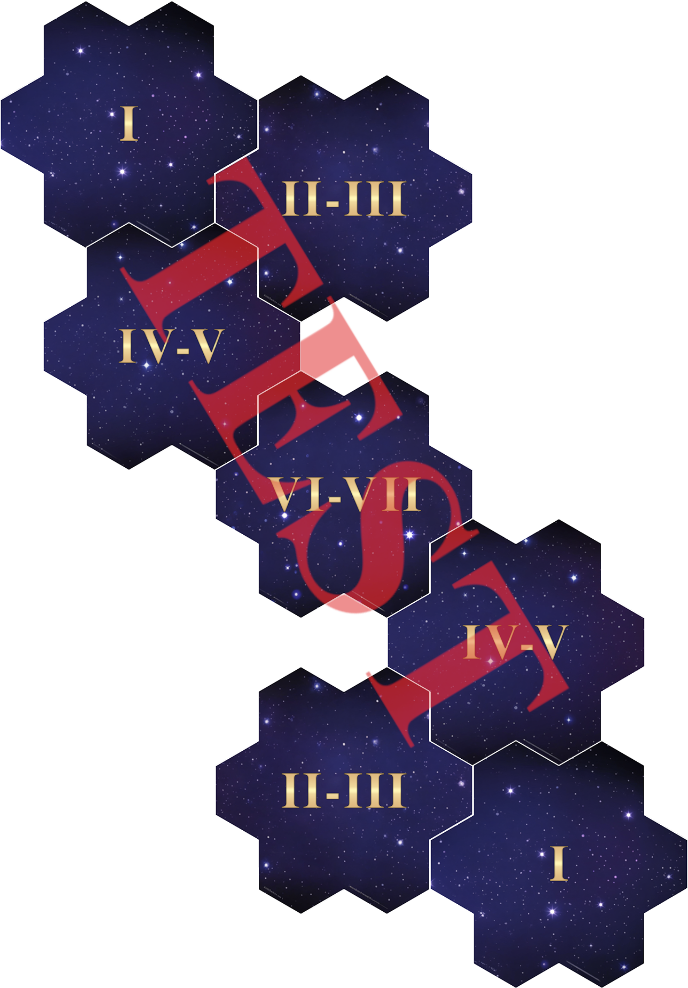
\includegraphics[width=\linewidth]{\_assets/maps/force-of-will-2p.png}};
  \node at (14, -3) {\footnotesize{\textbf{\MakeUppercase{2-PLAYER SCENARIO}}}};
  \node at (7, -7) {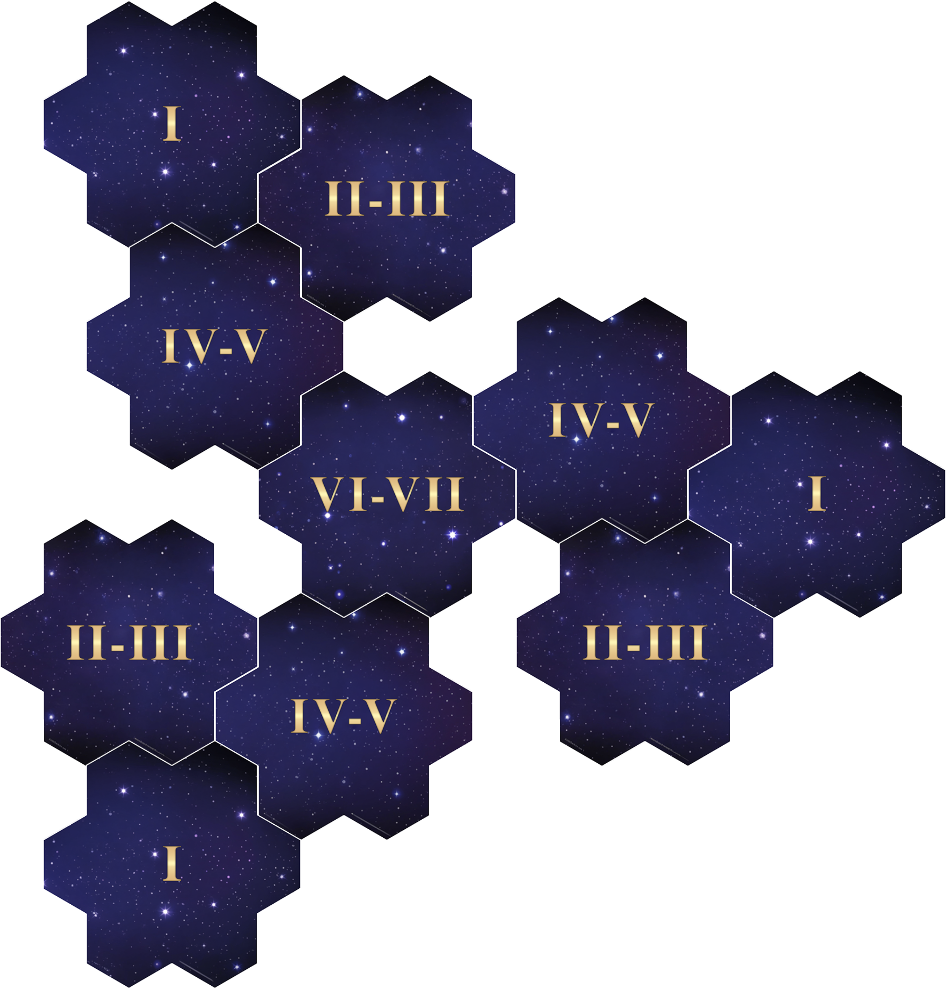
\includegraphics[width=1.35\linewidth]{\_assets/maps/force-of-will-3p.png}};
  \node at (7, -13.5) {\footnotesize{\textbf{\MakeUppercase{3-PLAYER SCENARIO}}}};
\end{tikzpicture}

\end{multicols*}
